% Robustness study section for tech report

\subsection{Designs and Quotas}

To assess whether the 48-tap base-case observation generalizes, five
FIR designs were tested under three proportional quotas each (15
design/quota combinations). The designs are:

\begin{itemize}
\item A: 48-tap, passband 0--0.3$\pi$, stopband 0.4$\pi$--$\pi$,
$-40$\,dB (base case)
\item B: 48-tap, same bands, $-50$\,dB stopband limit
\item C: 48-tap, passband 0--0.2$\pi$, stopband 0.3$\pi$--$\pi$,
$-40$\,dB (narrower transition)
\item D: 36-tap, same bands and limit as A (replaced the originally
planned 32-tap case, which did not meet $-40$\,dB as a floating-point
prototype)
\item E: 64-tap, same bands and limit as A
\end{itemize}

All five floating-point prototypes satisfy their stated passband and
stopband limits. Quotas are proportional to the 48-tap base case
($[24,16,8]$, $[16,24,8]$, $[12,24,12]$), scaled proportionally to the
tap count and adjusted to sum exactly to that count. Some scaled quotas
are odd (for example, $[22,32,10]$ for 64 taps).

\subsection{Results}

Table~\ref{tab:robust} reports the coefficient SSE and computed stopband
peak for each design/quota/method combination. DP and MILP coefficient-SSE
optima agree in every case.

\begin{table}[!t]
\caption{Robustness study: coefficient SSE and computed stopband peak}
\label{tab:robust}
\centering
\scriptsize
\resizebox{\columnwidth}{!}{%
\begin{tabular}{c l r r c c c}
\toprule
Case & Quota & DP SSE & Greedy SSE & DP stop (dB) & DP pass? & Greedy pass?\\
\midrule
A & $[24,16,8]$ & $1.86\!\cdot\!10^{-5}$ & $6.67\!\cdot\!10^{-5}$ & $-41.30$ & Yes & No\\
A & $[16,24,8]$ & $5.61\!\cdot\!10^{-5}$ & $1.07\!\cdot\!10^{-4}$ & $-35.32$ & No & No\\
A & $[12,24,12]$ & $9.93\!\cdot\!10^{-5}$ & $1.25\!\cdot\!10^{-4}$ & $-31.45$ & No & No\\
B & $[24,16,8]$ & $4.02\!\cdot\!10^{-5}$ & $8.42\!\cdot\!10^{-5}$ & $-35.55$ & No & No\\
B & $[16,24,8]$ & $9.35\!\cdot\!10^{-5}$ & $1.24\!\cdot\!10^{-4}$ & $-34.02$ & No & No\\
B & $[12,24,12]$ & $1.56\!\cdot\!10^{-4}$ & $1.56\!\cdot\!10^{-4}$ & $-32.42$ & No & No\\
C & $[24,16,8]$ & $5.47\!\cdot\!10^{-5}$ & $9.62\!\cdot\!10^{-5}$ & $-34.86$ & No & No\\
C & $[16,24,8]$ & $8.18\!\cdot\!10^{-5}$ & $1.16\!\cdot\!10^{-4}$ & $-35.32$ & No & No\\
C & $[12,24,12]$ & $1.32\!\cdot\!10^{-4}$ & $1.51\!\cdot\!10^{-4}$ & $-31.85$ & No & No\\
D & $[18,12,6]$ & $2.22\!\cdot\!10^{-5}$ & $2.22\!\cdot\!10^{-5}$ & $-35.60$ & No & No\\
D & $[12,18,6]$ & $5.94\!\cdot\!10^{-5}$ & $5.94\!\cdot\!10^{-5}$ & $-30.75$ & No & No\\
D & $[10,16,10]$ & $3.02\!\cdot\!10^{-4}$ & $3.02\!\cdot\!10^{-4}$ & $-28.16$ & No & No\\
E & $[32,22,10]$ & $2.20\!\cdot\!10^{-5}$ & $7.67\!\cdot\!10^{-5}$ & $-40.76$ & Yes & No\\
E & $[22,32,10]$ & $5.50\!\cdot\!10^{-5}$ & $8.08\!\cdot\!10^{-5}$ & $-36.78$ & No & No\\
E & $[16,32,16]$ & $8.68\!\cdot\!10^{-5}$ & $9.68\!\cdot\!10^{-5}$ & $-32.85$ & No & No\\
\bottomrule
\end{tabular}}
\end{table}

\begin{figure*}[!t]
\centering
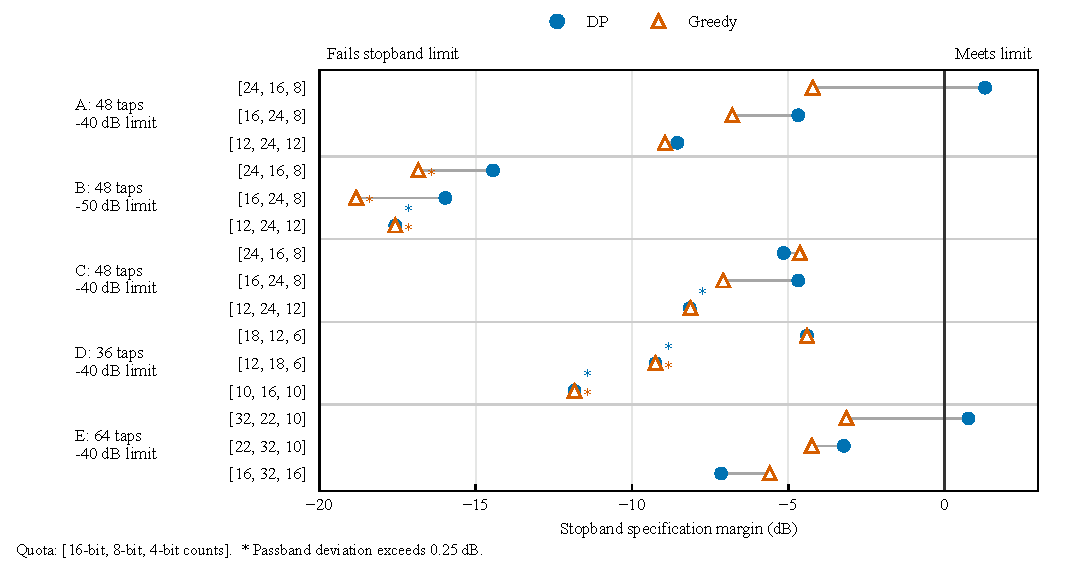
\includegraphics[width=\textwidth]{figures/robustness_margin.pdf}
\caption{All 15 design/quota combinations, using computed responses.
Margin is the specified stopband upper limit minus the computed stopband
peak; nonnegative values meet the stopband limit. Case B uses $-50$\,dB;
the other cases use $-40$\,dB. Asterisks mark passband deviations exceeding
$0.25$\,dB. Hollow greedy triangles keep coincident DP markers visible.
DP meets both limits in 2/15 combinations; greedy in 0/15.
These are software results, not hardware measurements.}
\label{fig:robust-margin}
\end{figure*}

\subsection{Interpretation}

Figure~\ref{fig:robust-margin} shows the stopband margin for every tested
combination and flags passband violations. DP meets both response limits
in 2 of 15 combinations; greedy meets
them in 0. The two DP passes occur for the highest-precision quota in
cases A and E. This is not a universal frequency-response advantage:
in case C's first quota, greedy has a slightly lower stopband peak
($-35.37$ vs.\ $-34.86$\,dB), although both fail the $-40$\,dB limit.

Lower coefficient SSE does not imply lower stopband peak or compliance
with a response specification. These results support a bounded
observation about five prototypes and three proportional quotas only;
they do not establish general performance claims. All results are
software frequency-response calculations; the 36- and 64-tap designs
were not synthesized, routed, or tested on hardware.
